% LaTeX document: display three images and append the Python code
% Save as report.tex. Place Figure_1.png, Figure_2.png, Figure_3.png in the same folder.
\documentclass{article}
\usepackage[margin=1in]{geometry}
\usepackage{graphicx}
\usepackage{caption}
\usepackage{listings}
\usepackage{xcolor}


\lstset{
  language=Python,
  basicstyle=\ttfamily\small,
  keywordstyle=\color{blue},
  commentstyle=\color{gray},
  stringstyle=\color{teal},
  breaklines=true,
  columns=fullflexible,
  showstringspaces=false
}

\title{EE604 H5}
\author{LOHIT P TALAVAR \\ 210564 \\ \texttt{lohitpt21@iitk.ac.in}}
\date{\today}

\begin{document}

\maketitle

% --- Three images (only images shown) ---
\begin{figure}[htp]
  \centering
  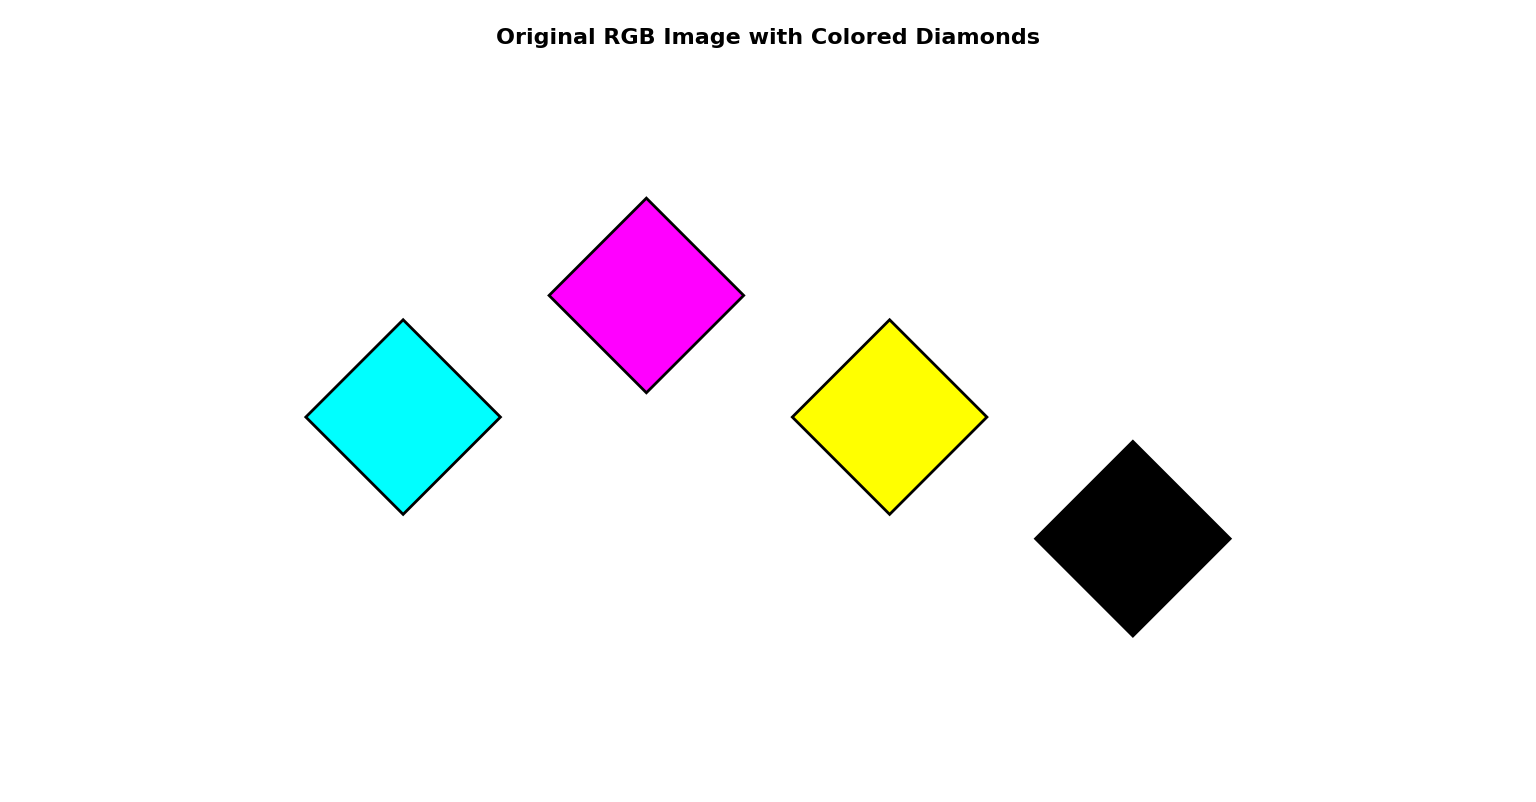
\includegraphics[width=0.9\textwidth]{Figure_1.png}
  \vspace{6pt}
\end{figure}

\begin{figure}[htp]
  \centering
  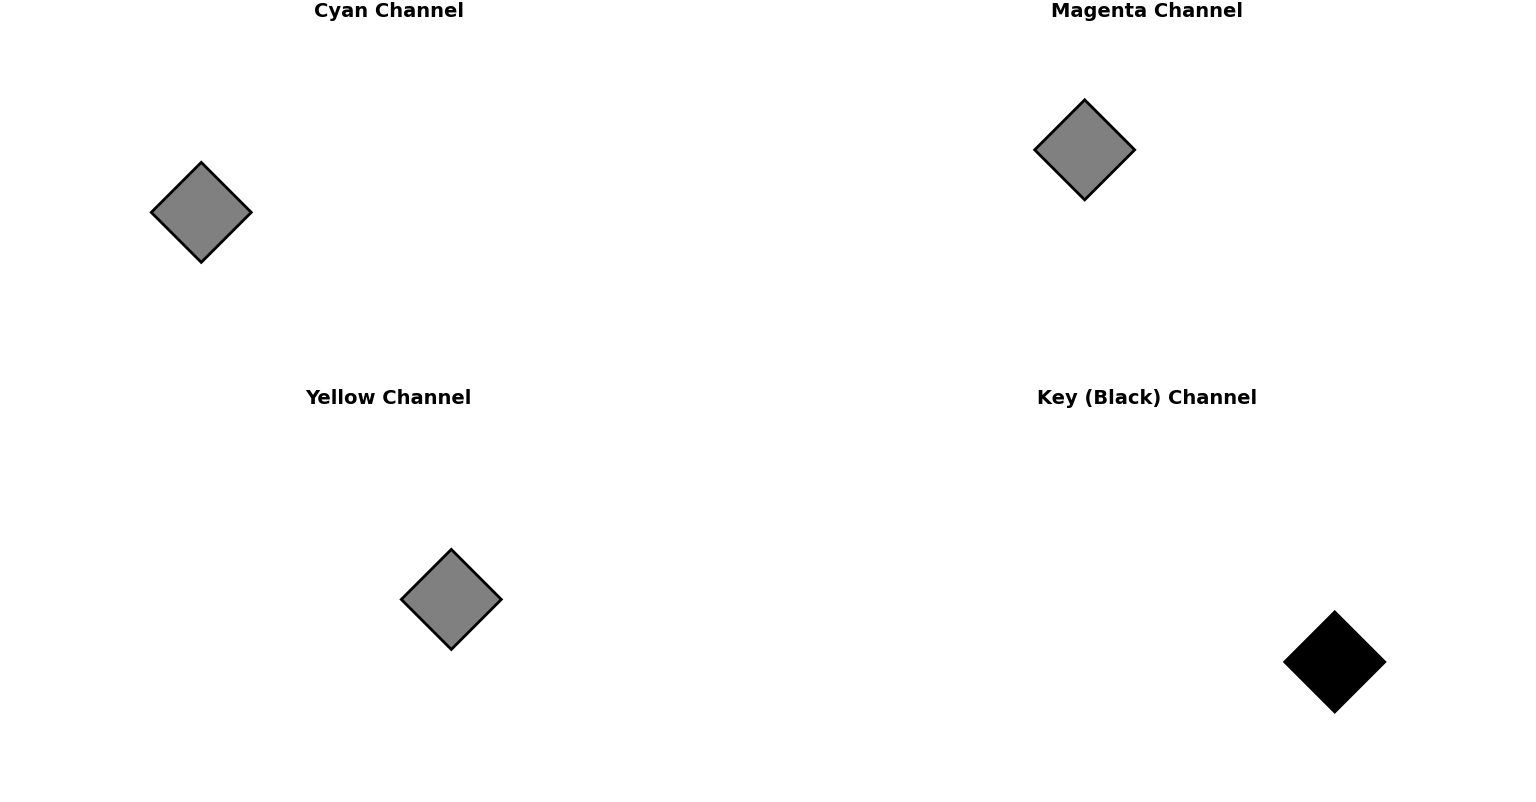
\includegraphics[width=0.9\textwidth]{Figure_2.png}
  \vspace{6pt}
\end{figure}

\begin{figure}[htp]
  \centering
  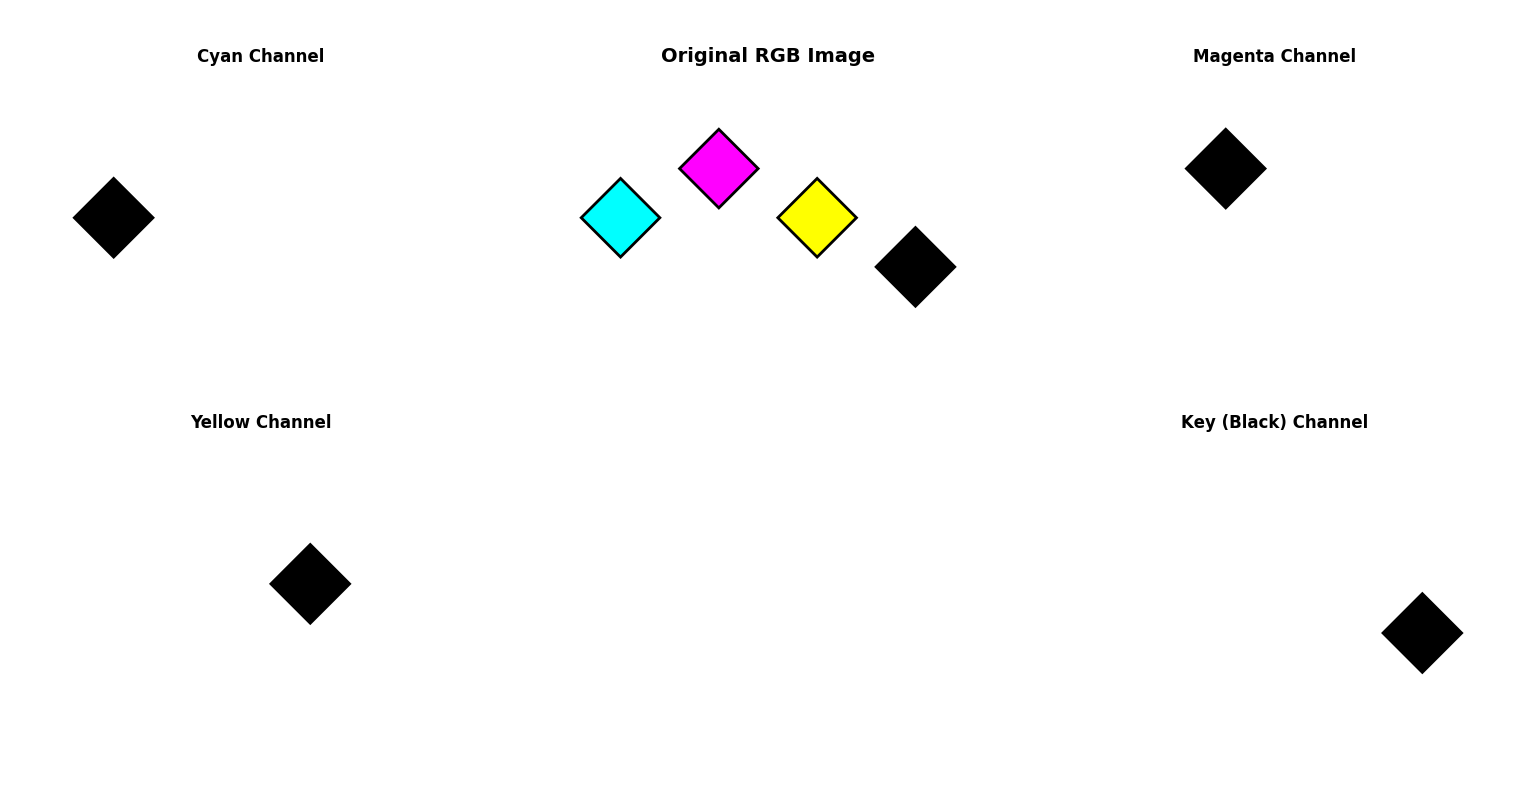
\includegraphics[width=0.9\textwidth]{Figure_3.png}
  \vspace{6pt}
\end{figure}

\clearpage
% --- Append the Python code ---
\section*{Python code}
\begin{lstlisting}
import numpy as np
import matplotlib.pyplot as plt
from matplotlib.patches import Polygon
from matplotlib.colors import ListedColormap

def create_diamond_vertices(center_x, center_y, size):
    """Create vertices for a diamond (rhombus) shape"""
    return np.array([
        [center_x, center_y + size],  # top
        [center_x + size, center_y],  # right
        [center_x, center_y - size],  # bottom
        [center_x - size, center_y]   # left
    ])

def rgb_to_cmyk(r, g, b):
    """Convert RGB values to CMYK"""
    # Normalize RGB to 0-1 range
    r, g, b = r/255.0, g/255.0, b/255.0
    
    # Calculate K (black)
    k = 1 - max(r, g, b)
    
    # Calculate CMY
    if k == 1:
        c = m = y = 0
    else:
        c = (1 - r - k) / (1 - k)
        m = (1 - g - k) / (1 - k)
        y = (1 - b - k) / (1 - k)
    
    return c, m, y, k

def create_rgb_image():
    """Create the original RGB image with four colored diamonds"""
    fig, ax = plt.subplots(1, 1, figsize=(10, 6))
    
    # Set white background
    ax.set_xlim(0, 10)
    ax.set_ylim(0, 6)
    ax.set_facecolor('white')
    
    # Diamond positions and colors
    diamonds = [
        {'pos': (2, 3), 'color': 'cyan', 'rgb': (0, 255, 255)},
        {'pos': (4, 4), 'color': 'magenta', 'rgb': (255, 0, 255)},
        {'pos': (6, 3), 'color': 'yellow', 'rgb': (255, 255, 0)},
        {'pos': (8, 2), 'color': 'black', 'rgb': (0, 0, 0)}
    ]
    
    diamond_size = 0.8
    
    # Draw each diamond
    for diamond in diamonds:
        vertices = create_diamond_vertices(diamond['pos'][0], diamond['pos'][1], diamond_size)
        polygon = Polygon(vertices, closed=True, facecolor=diamond['color'], 
                         edgecolor='black', linewidth=2)
        ax.add_patch(polygon)
    
    ax.set_aspect('equal')
    ax.set_title('Original RGB Image with Colored Diamonds', fontsize=16, fontweight='bold')
    ax.axis('off')
    
    plt.tight_layout()
    plt.show()
    
    return diamonds, diamond_size

def create_cmyk_channels(diamonds, diamond_size):
    """Create CMYK channel separation images"""
    fig, axes = plt.subplots(2, 2, figsize=(12, 8))
    axes = axes.flatten()
    
    channel_names = ['Cyan Channel', 'Magenta Channel', 'Yellow Channel', 'Key (Black) Channel']
    channel_colors = ['cyan', 'magenta', 'yellow', 'black']
    
    for i, (ax, channel_name, channel_color) in enumerate(zip(axes, channel_names, channel_colors)):
        # Set white background
        ax.set_xlim(0, 10)
        ax.set_ylim(0, 6)
        ax.set_facecolor('white')
        
        # Draw diamonds - only show the one corresponding to this channel
        for diamond in diamonds:
            if diamond['color'] == channel_color:
                vertices = create_diamond_vertices(diamond['pos'][0], diamond['pos'][1], diamond_size)
                
                # For better visualization of channels, use grayscale
                # Darker = more ink in that channel
                if channel_color == 'black':
                    fill_color = 'black'
                else:
                    fill_color = 'gray'
                
                polygon = Polygon(vertices, closed=True, facecolor=fill_color, 
                                edgecolor='black', linewidth=2)
                ax.add_patch(polygon)
        
        ax.set_aspect('equal')
        ax.set_title(channel_name, fontsize=14, fontweight='bold')
        ax.axis('off')
    
    plt.tight_layout()
    plt.show()

def demonstrate_cmyk_conversion():
    """Demonstrate CMYK conversion with numerical values"""
    print("RGB to CMYK Conversion Values:")
    print("=" * 50)
    
    colors = [
        ('Cyan', 0, 255, 255),
        ('Magenta', 255, 0, 255),
        ('Yellow', 255, 255, 0),
        ('Black', 0, 0, 0)
    ]
    
    for color_name, r, g, b in colors:
        c, m, y, k = rgb_to_cmyk(r, g, b)
        print(f"{color_name}:")
        print(f"  RGB: ({r}, {g}, {b})")
        print(f"  CMYK: C={c*100:.0f}% M={m*100:.0f}% Y={y*100:.0f}% K={k*100:.0f}%")
        print()

def create_advanced_visualization():
    """Create a more detailed visualization showing actual CMYK values"""
    fig, axes = plt.subplots(2, 3, figsize=(15, 10))
    
    # Original RGB image
    ax_rgb = axes[0, 1]
    ax_rgb.set_xlim(0, 10)
    ax_rgb.set_ylim(0, 6)
    ax_rgb.set_facecolor('white')
    
    diamonds = [
        {'pos': (2, 3), 'color': 'cyan', 'rgb': (0, 255, 255)},
        {'pos': (4, 4), 'color': 'magenta', 'rgb': (255, 0, 255)},
        {'pos': (6, 3), 'color': 'yellow', 'rgb': (255, 255, 0)},
        {'pos': (8, 2), 'color': 'black', 'rgb': (0, 0, 0)}
    ]
    
    diamond_size = 0.8
    
    # Draw diamonds on RGB image
    for diamond in diamonds:
        vertices = create_diamond_vertices(diamond['pos'][0], diamond['pos'][1], diamond_size)
        polygon = Polygon(vertices, closed=True, facecolor=diamond['color'], 
                         edgecolor='black', linewidth=2)
        ax_rgb.add_patch(polygon)
    
    ax_rgb.set_aspect('equal')
    ax_rgb.set_title('Original RGB Image', fontsize=14, fontweight='bold')
    ax_rgb.axis('off')
    
    # CMYK channels
    channel_positions = [(0, 0), (0, 2), (1, 0), (1, 2)]
    channel_names = ['Cyan', 'Magenta', 'Yellow', 'Key (Black)']
    channel_colors = ['cyan', 'magenta', 'yellow', 'black']
    
    for pos, name, color in zip(channel_positions, channel_names, channel_colors):
        ax = axes[pos]
        ax.set_xlim(0, 10)
        ax.set_ylim(0, 6)
        ax.set_facecolor('white')
        
        # Draw only the diamond corresponding to this channel
        for diamond in diamonds:
            if diamond['color'] == color:
                vertices = create_diamond_vertices(diamond['pos'][0], diamond['pos'][1], diamond_size)
                
                # Show intensity based on CMYK value
                r, g, b = diamond['rgb']
                c, m, y, k = rgb_to_cmyk(r, g, b)
                
                if name == 'Cyan':
                    intensity = c
                elif name == 'Magenta':
                    intensity = m
                elif name == 'Yellow':
                    intensity = y
                else:  # Key (Black)
                    intensity = k
                
                # Convert intensity to grayscale (0 = white, 1 = black)
                gray_value = 1 - intensity
                fill_color = (gray_value, gray_value, gray_value)
                
                polygon = Polygon(vertices, closed=True, facecolor=fill_color, 
                                edgecolor='black', linewidth=2)
                ax.add_patch(polygon)
        
        ax.set_aspect('equal')
        ax.set_title(f'{name} Channel', fontsize=12, fontweight='bold')
        ax.axis('off')
    
    # Remove empty subplot
    axes[1, 1].axis('off')
    
    plt.tight_layout()
    plt.show()

def main():
    """Main function to run the complete demonstration"""
    print("RGB to CMYK Diamond Shape Converter")
    print("=" * 40)
    print()
    
    # Show numerical conversion
    demonstrate_cmyk_conversion()
    
    # Create and display images
    print("Creating RGB image with colored diamonds...")
    diamonds, diamond_size = create_rgb_image()
    
    print("Creating CMYK channel separation...")
    create_cmyk_channels(diamonds, diamond_size)
    
    print("Creating advanced visualization...")
    create_advanced_visualization()
    
    print("Process completed! All images have been displayed and saved.")
    print("\nSaved files:")
    print("- rgb_diamonds_original.png (Original RGB image)")
    print("- cmyk_channels_combined.png (All CMYK channels together)")
    print("- cmyk_cyan_channel.png (Cyan channel only)")
    print("- cmyk_magenta_channel.png (Magenta channel only)")
    print("- cmyk_yellow_channel.png (Yellow channel only)")
    print("- cmyk_black_channel.png (Black channel only)")
    print("- cmyk_advanced_visualization.png (Complete visualization)")
    
    print("\nAll images are saved at 300 DPI with white background for homework submission.")

# Run the program
if __name__ == "__main__":
    main()
\end{lstlisting}

\end{document}
